
\documentclass[../main.tex]{subfiles}
\begin{document}
\chapter{Modélisation du métabolisme: d'une cellule à un écosystème}
\minitoc
\label{ch:edla}

\newpage

\section{Les modèles du métabolisme comme support de l'analyse microbienne}

\subsection{Reconstruction de réseaux métaboliques}
Le \textit{métabolisme} décrit toutes les réactions biochimiques au sein d'un organisme permettant de produire de l'énergie, de dégrader et de produire du matériel métabolique \citep{Nava2023}. Un moyen de le représenter est d'utiliser le \textit{réseau métabolique}. Un réseau métabolique décrit l'ensemble des voies métaboliques, composé d'une succession de réactions biochimiques, ainsi que les inter-connections entre ces voies, mises en avant par des métabolites en communs \citep{Goldford2018}. Le réseau métabolique est souvent utilisé par les biologistes leur permettant principalement d'identifier les voies métaboliques. Pour effectuer des simulations numériques ou étudier la topologie du réseau, le réseau métabolique est utilisé dans des modèles mathématiques ou informatiques dits \textit{modèle métabolique}.\\

Afin d'illustrer ce que sont que les réactions métaboliques, nous allons prendre l'exemple du processus de photosynthèse. Les plantes utilise l'énergie du soleil, \textit{i.e.} la lumière, pour le convertir en sucre, comme le glucose, et en di-oxyde de carbone ($\text{CO}_2$), par la réaction anabolique suivante:

\[
\text{reaction}_\text{anabolique} : 6\text{CO}_2 + 6\text{H}_2\text{O} + \text{energie} \rightarrow \text{glucose} + 6\text{O}_2
\]

La réaction est dite anabolique lorsqu'elle produit de grosses molécules à partir de plus petites, et de l'énergie, sous forme de molécules d'ATP par exemple, est nécessaire. Tandis que les réactions cataboliques sont responsables du processus inverse, et libèrent donc de l'énergie. La réaction catabolique de $\text{reaction}_\text{anabolique}$ représentant le processus de respiration est:

\[
\text{reaction}_\text{catabolique} : \text{glucose} + 6\text{O}_2\rightarrow 6\text{CO}_2 + 6\text{H}_2\text{O} + \text{energie} 
\]

Ainsi, les voies métaboliques sont constituées de multiples réactions anaboliques et cataboliques, comme illustrées par la figure \ref{fig:metabolic-pathways} qui représente l'ensemble des voies métaboliques de la bactérie \textit{E. coli}.

\begin{figure}[H]
    \centering
    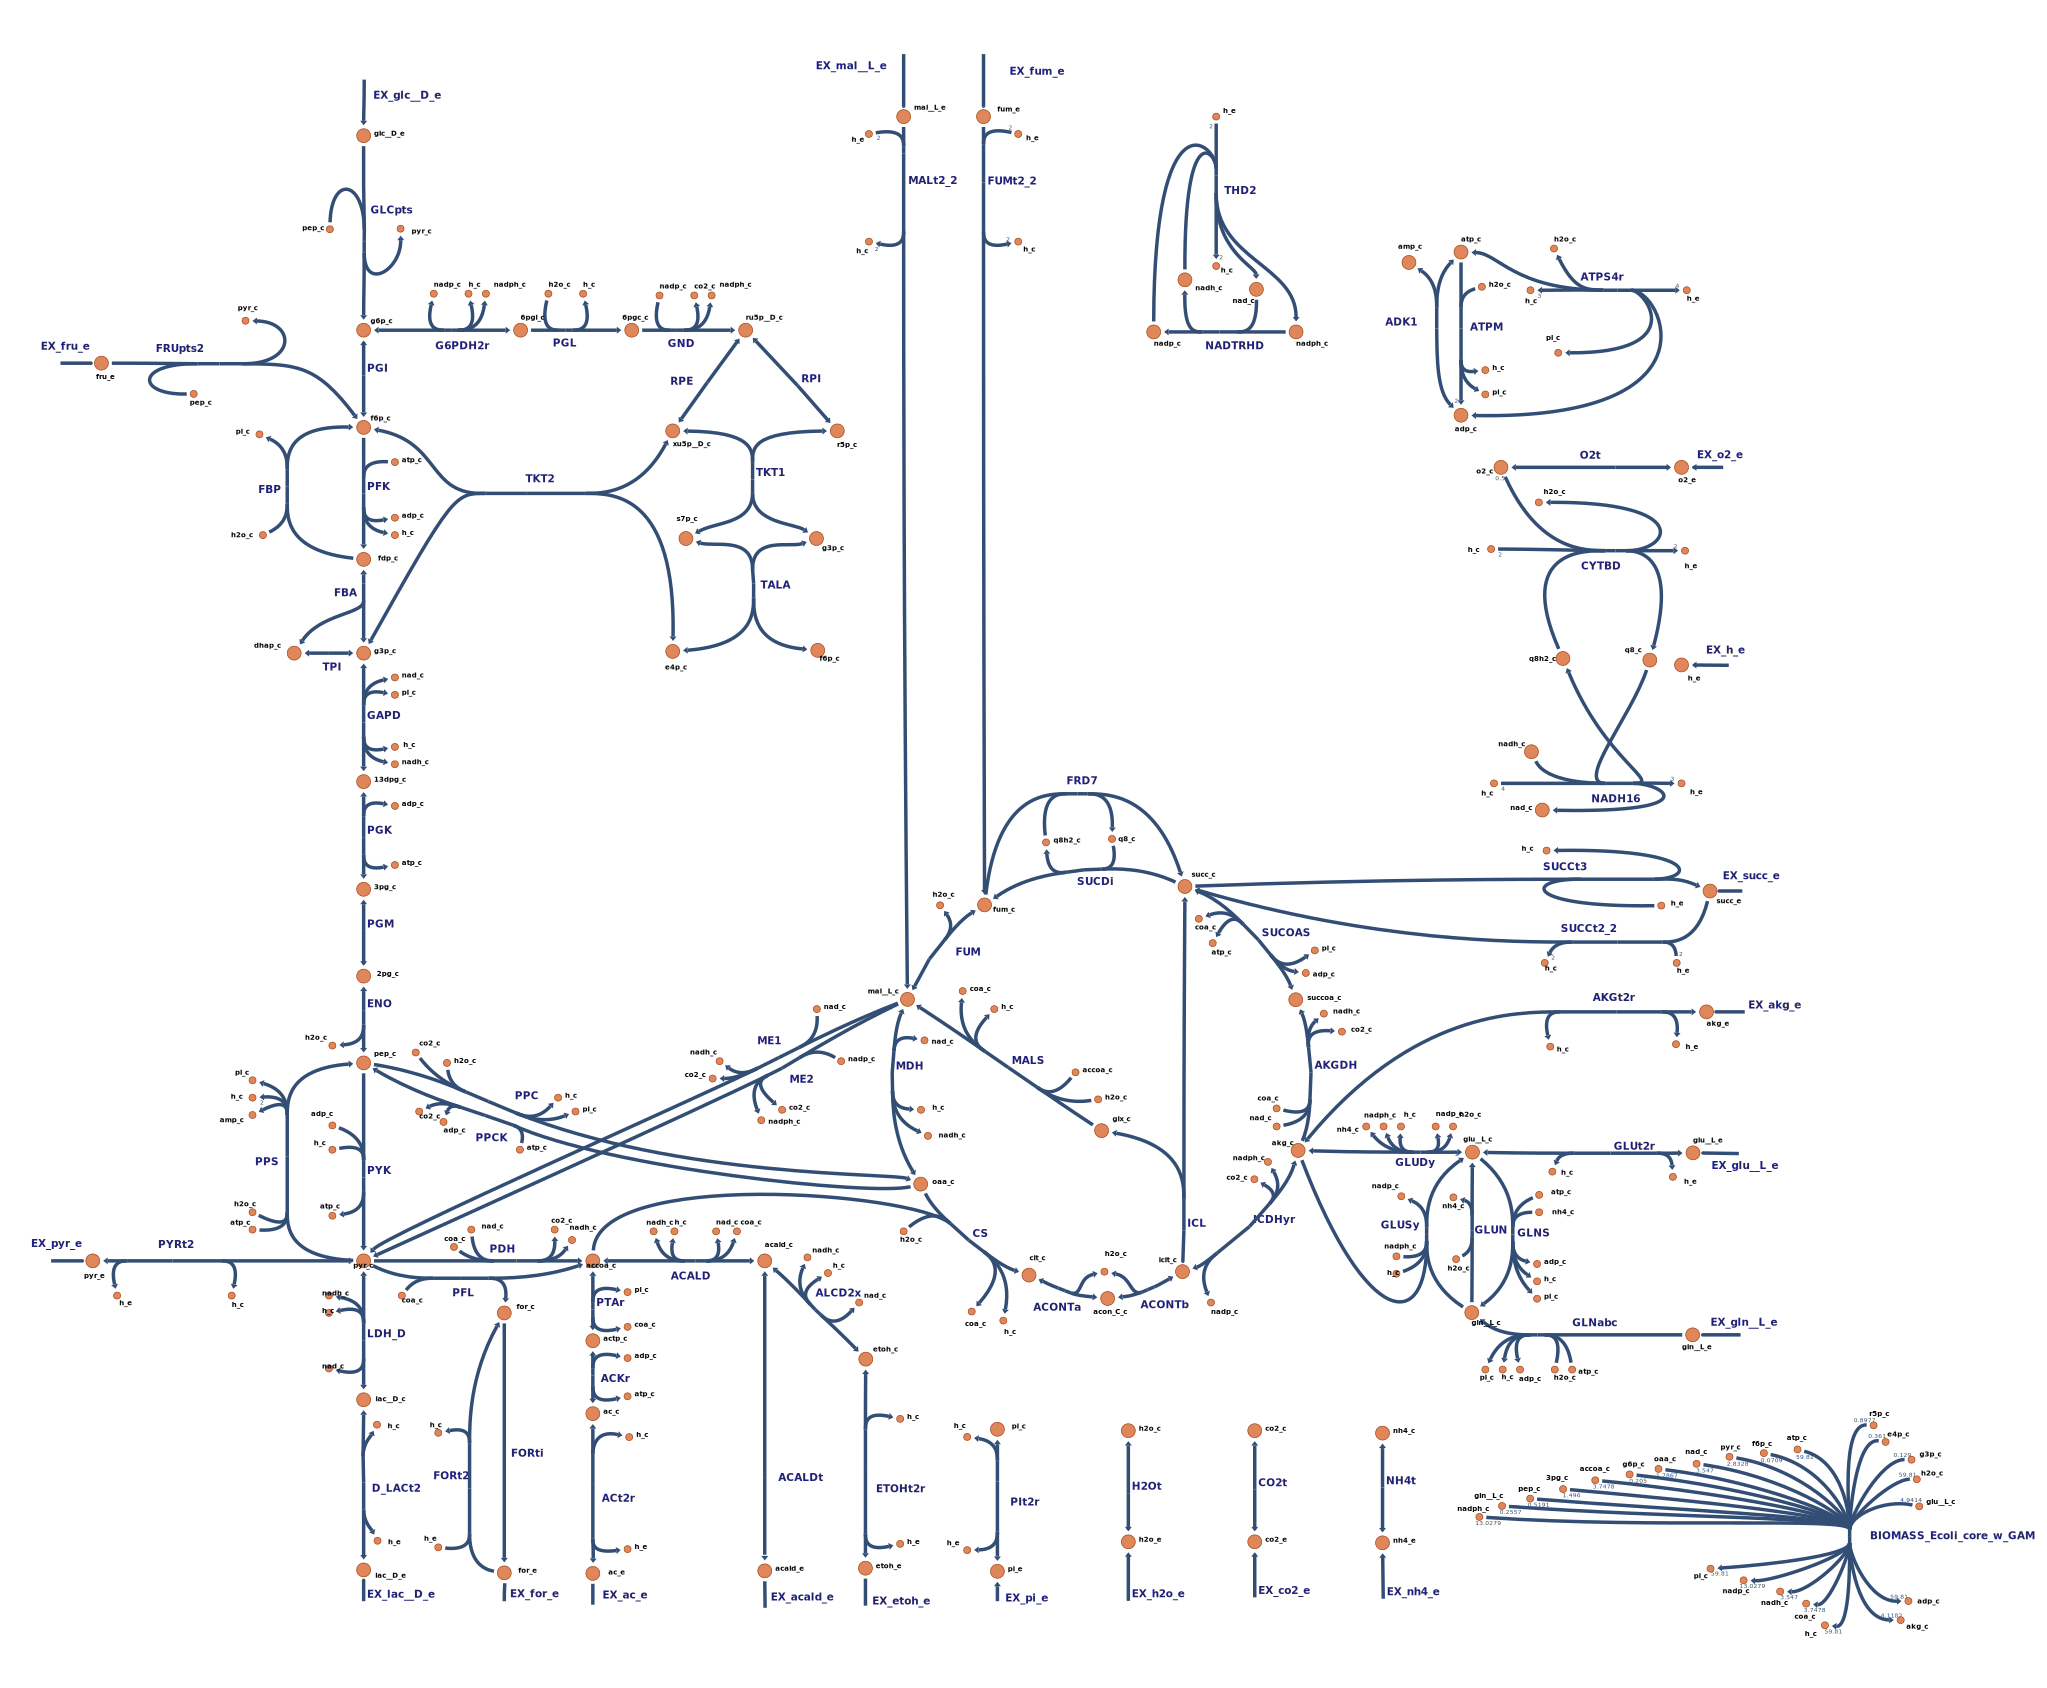
\includegraphics[width=\textwidth]{img/EDLA/metabolic-pathway-ecoli.pdf}
    \caption{Illustration des voies métaboliques de \textit{E. coli} dans l'application web Escher \citep{King2015}}
    \label{fig:metabolic-pathways}
\end{figure}

Enfin, par convention, le plus petit réseau métabolique sur lequel une analyse peut être faite est constitué d'une réaction de production et d'une réaction de consommation. Chez la bactérie, on retrouve des réseaux métaboliques allant de quelques réactions à plus de deux mille dans le cas des réseaux métaboliques à l'échelle du génome, et peut atteindre plus de dix mille réactions dans le cas du réseau métabolique humain \citep{Robinson2020}.

Un réseau métabolique se caractérise par l'association de gènes à des protéines qui catalysent des réactions (GPR) \cite{Thiele.2010}. Ces associations se basent sur des règles d'association booléennes entre les gènes et les réactions. Considérons les réactions $r1$, $r2$ associées aux gènes $g1$, $g2$, $g3$ par les relations logiques suivantes:

\begin{align}
\label{gpr1}
    r1 : (g1 \land g2) \lor (g1 \land g3)
\end{align}
\begin{align}
\label{gpr2}
    r2 : g1 \land (g2 \lor g3)
\end{align}

La règle booléenne \ref{gpr1} stipule que, pour que la réaction $r1$ soit activée, il faut que le complexe $g1$ et $g2$ soit exprimé ou que le complexe $g1$ et $g3$ soit exprimé. Dans le cas de la règle d'association \ref{gpr2}, la réaction $r2$ est activée si $g1$ est exprimé avec $g2$ ou $g3$. Dans ce cas précis, si seul $g2$ ou $g3$ est exprimé mais que $g1$ ne l'est pas, alors la réaction $r2$ ne pourra pas être catalysée \\

Afin de reconstruire le réseau métabolique, un génome annoté est nécessaire. A partir d'une séquence génomique d'un organisme, deux annotations du génome sont possibles \citep{Médigue2002} : structurelle, permettant d'identifier les gènes (par exemple, AUGUSTUS \citep{Nachtweide2019}, Glimmer \citep{Delcher2007}), et  fonctionnelle, pour retrouver la biochimie et les fonctions biologiques portées par une protéine (par exemple, Blast \citep{Altschul1990}, par un processus d'alignement). Un grand panel de bases de données existe permettant une annotation à plusieurs échelles du génome. Il existe BRENDA \citep{Chang2021} se concentrant sur les enzymes et les données liées au métabolisme ou encore EggNOG se focalisant sur une annotation fonctionnelle \cite{Huerta-Cepas2019}. Des outils utilisant les différentes bases de données existent comme exemple Eggnog-mapper \citep{Cantalapiedra2021}, Rast \citep{Aziz2008}, Prokka \citep{Seemann2014} ou encore MicrosCope \citep{Vallenet2020} .\\


Le génome étant annoté, le réseau métabolique peut-être reconstruit manuellement et/ou automatiquement avec une approche ascendante (bottom-up) et/ou une approche descendante (top-down), en utilisant une large collection d'outils \citep{Mendoza2019} (voir Figgure \ref{fig:approche-reconstruction}. Tous les outils de reconstruction utilisent une base de données leur permettant d'assigner une fonction métabolique portée par un gène. Les approches bottom-up se caractérisent par un processus itératif de génération d'ébauches de réseaux métaboliques suivi de curation tandis que les approches descendantes, sont définies par la production de réseaux métaboliques "prêts à l'emploi". Dans ce deuxième cas, les fonctions assignées dans les modèles métaboliques gardent la curation d'un modèle universel fonctionnels, leur assurant ainsi une bonne qualité dû à leur faible nombre d'assignation faux-positif. \\


Parmi les deux approches, on retrouve GEMSiRV \citep{Liao2012}, CarveME \citep{Machado2018} et MetaDraft \citep{olivier2018} qui représentent les outils utilisant l'approche descendante. Les deux derniers outils se servent de la base de données BIGG \citep{King2016} pour construire leurs modèles universels. Une plus grande bibliographie existe concernant l'approche ascendante avec FAME \citep{Boele2012}, CoReCo \citep{Pitkanen2014}, Merlin \citep{Dias2015}, RAVEN \citep{Wang2018} et autoKEGGRec \citep{Karlsen2018} se reposant sur la base de données KEGG \citep{Kanehisa}. Pathway-tools \citep{Karp2022} ou encore AuReMe \citep{Aite2018}, tous deux basés sur la base de données MetaCyc \citep{Caspi2018}, ModelSEED \citep{Seaver2021} et Kbase \citep{Arkin2018} ou encore gapSeq \citep{Zimmermann2021}. L'outil rBioNet \citep{Thorleifsson2011}, allie à la fois la reconstruction descendante et ascendante, permettant à l'utilisateur ou l'utilisatrice de créer elle même son réseau métabolique ou d'en importer un sur lequel elle peut se baser pour le reconstruire. \\


\begin{figure}[H]
    \centering
    \includegraphics[width=\textwidth]{img/EDLA/approche-bottom-up-top-down.pdf}
    \caption{Illustration des approches descendante (a) et ascendante (b) pour reconstruire des modèles métaboliques à l'échelle du génome fonctionnels. En (a), la partie de curation manuelle n'est pas prise en compte dans l'approche de reconstruction, ce qui n'est pas le cas de l'approche ascendante (b). \maxime{texte trop petit ?} }
    \label{fig:approche-reconstruction}
\end{figure}



\subsubsection*{Diffusion et qualité des réseaux métabolique}
On peut voir qu'il existe plusieurs outils permettant de reconstruire le métabolisme. Cependant, standardiser sa représentation n'est pas encore acquis par la communauté scientifique \citep{Stobbe2014}. En effet, chaque base de données possède les fichiers de sortie différents permettant la représentation de la connaissance du métabolisme. On peut retrouver par exemple, BioCyc \citep{Karp2018} qui utilise des fichiers plats PGDB, le format BioPAX \citep{Demir2010} ou encore SBML\citep{Hucka2019}. La base de données KEGG \citep{Kanehisa} utilise d'autres fichiers plats et sa propre façon de représenter le métabolisme : KEGG Markup Language. Même si le choix syntaxique utilisé n'est pas commun à touts, nous retrouvons majoritairement le format SBML pour Systeme Biology Markup Language \citep{Hucka2019}, qui permet de représenter les voies de signalisation mais également, des paramètres mathématiques utiles pour la modélisation.

Concernant l'évaluation de la qualité du réseaux métabolique, au delà de l'objectif même de l'utilisateur ou de l'utilisatrice, il existe MEMOTE \citep{Lieven.2020} capable de vérifier la consistance du réseau métabolique en terme du nombre de gènes associés à des réactions, le nombre de réactions non associées à au moins un gène ou encore le nombre de métabolites qui ne sont jamais consommés mais produits, et donc, étant en accumulation dans le système. Le score évaluant la qualité du réseau est borné par la méthode de reconstruction choisie \citep{Lieven.2020}.


\subsection{Représentations mathématiques et informatiques du métabolisme}
Le métabolisme peut se représenter de deux grandes façons : sous forme d'un hypergraphe dirigé simple ou bipartite \citep{Belcour.2020}, ou sous forme d'une matrice st\oe{}chiométrique. La représentation sous forme d'un graphe informe sur les liens entre les réactions et métabolites d'un système biologique plutôt que sur la quantité de métabolites produits et/ou consommé associée davantage à la matrice st\oe{}chiométrique. Nous allons prendre l'exemple d'une voie de production connue, la glycolyse, chez une espèce lactique : \textit{Lactiplantibacillus plantarum}\\

Représentation simplifiée de la glycolyse chez \textit{Lactiplantibacillus plantarum}:\\
( HEX1 ) : $1\text{ glucose} \rightarrow 1\text{ glucose-6-phosphate}$\\
( PGI ) : $1\text{ glucose-6-phosphate} \leftrightarrow 1\text{ fructose-6-phosphate} $\\
( PFK ) : $1\text{ fructose-6-phosphate} \rightarrow 1\text{ D-Fructose 1,6-bisphosphate}$  \\
( FBA ) : $1\text{ D-Fructose 1,6-bisphosphate} \leftrightarrow 1\text{ Dihydroxyacetone phosphate}$\\$ + 1\text{ Glyceraldehyde 3-phosphate} $\\
( GAPD ) : $1\text{ Glyceraldehyde 3-phosphate}  \leftrightarrow 1\text{ 3-Phospho-D-glyceroyl phosphate} $\\
( PGK ) : $1\text{ 3-Phospho-D-glycerate} \leftrightarrow 1\text{ 3-Phospho-D-glyceroyl phosphate} $\\
( PGM ) : $1\text{ 3-Phospho-D-glycerate} \leftrightarrow  1\text{ 2-Phospho-D-glycerate} $\\
( ENO ) : $1\text{ 2-Phospho-D-glycerate} \leftrightarrow 1\text{ Phosphoenolpyruvate} $\\
( PYK ) : $1\text{ Phosphoenolpyruvate} \rightarrow 1\text{ pyruvate}$ \\

où $\text{HEX1}$, $\text{PGI}$, $\text{PFK}$, $\text{FBA}$, $\text{GAPD}$, $\text{PGK}$, $\text{PGM}$, $\text{ENO}$, $\text{PYK}$ sont les ensembles de réactions et où $\text{glucose}$, $\text{glucose-6-phosphate}$, $\text{fructose-6-phosphate}$, $\text{D-Fructose 1,6-bisphosphate}$, $\text{Dihydroxyacetone phosphate}$, $\text{Glyceraldehyde 3-phosphate}$, $\text{3-Phospho-D-glyceroyl phosphate}$, $\text{3-Phospho-D-glycerate}$, $\text{2-Phospho-D-glycerate}$, $\text{Phosphoenolpyruvate}$ et $\text{ pyruvate}$ sont les ensembles de métabolites principaux constituants la glycolyse de \textit{Lactiplantibacillus plantarum}.


\subsubsection{Matrice st\oe{}chiométrique}
Le métabolisme peut-être représenté sous forme d'une matrice st\oe{}chiométrique dont l'ensemble des réactions et des métabolites du système constituent respectivement les colonnes et les lignes. Le nombre à l'intérieur de la matrice représente le coefficient st\oe{}chiométrique de la réaction biochimique. Ainsi, la glycolyse chez \textit{Lactiplantibacillus plantarum} est représentée par la matrice st\oe{}chiométrique  suivante: 

\renewcommand{\kbldelim}{(}% Left delimiter
\renewcommand{\kbrdelim}{)}% Right delimiter
\[
  \kbordermatrix{
     & \text{HEX1} & \text{PGI} & \text{PFK} & \text{FBA} & \text{GAPD} & \text{PGK} & \text{PGM} & \text{ENO} & \text{PYK} \\
    \text{glucose}                                           & -1 & 0 & 0 & 0 & 0 & 0 & 0 & 0 & 0 \\
    \text{glucose-6-phosphate}                      & 1 & -1 & 0 & 0 & 0 & 0 & 0& 0 & 0 \\
    \text{fructose-6-phosphate}                      & 0 & 1 & -1 & 0 & 0 & 0 & 0& 0 & 0  \\
    \text{D-Fructose 1,6-bisphosphate}          & 0 & 0 & 1 & -1& 0 & 0 & 0& 0 & 0  \\
    \text{Dihydroxyacetone phosphate}         & 0 & 0 & 0 & 1 & -1 & 0 & 0& 0 & 0  \\
    \text{Glyceraldehyde 3-phosphate}         & 0 & 0 & 0 & 1 & -1 & 0 & 0& 0 & 0  \\
    \text{3-Phospho-D-glyceroyl phosphate} & 0 & 0 & 0 & 0 & 1 & -1 & 0& 0 & 0  \\
    \text{3-Phospho-D-glycerate}                   & 0 & 0 & 0 & 0 & 0 & 1 & -1& 0 & 0 \\
    \text{2-Phospho-D-glycerate}                  & 0 & 0 & 0 & 0 & 0 & 0 & 1& -1 & 0  \\
    \text{Phosphoenolpyruvate}                    & 0 & 0 & 0 & 0 & 0 & 0 & 0& 1 & -1  \\
    \text{ pyruvate}                                         & 0 & 0 & 0 & 0 & 0 & 0 & 0& 0 & 1 \\
    }
\]


\subsubsection{Graphe}
Pour représenter des réseaux métaboliques, un graphe bipartite dirigé pondéré est souvent privilégié \citep{Barabasi2004}. Le graphe est alors composé de deux types de sommets, un pour les métabolites et un pour les réactions, et d'arcs symbolisant les relations "être produit par" ou "être consommé par" entre les métabolites et les réactions. Mathématiquement, il peut être exprimé ainsi : soit un graphe bipartite G définit comme un tuple $\gmodel = \langle M, R, E \rangle$ où $R$, $M$ et $E$ représentent les ensembles respectifs de réactions, de métabolites et des arcs reliant les métabolites aux réactions. Un réactant $m$ consommé par la réaction $r$ est définie comme $e = \langle m,r \rangle$, et un produit $m$ de la réaction $r$ est définie comme suit $e = \langle m,r \rangle$ où $m\in M$ et $r\in R $.

Une représentation de la glycolyse de \textit{Lactiplantibacillus plantarum} sous forme d'un graphe bipartite est illustrée dans la figure \ref{fig:graph-network}, où les carrés représentent les réactions et les cercles représentes les métabolites.


\begin{figure}[h!]
    \centering
    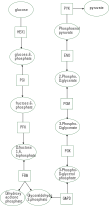
\includegraphics[width=0.6\textwidth]{img/EDLA/graph_network.pdf}
    \caption{Représentation du métabolisme sous forme d'un graphe bi-partite. Les carrés sont associés aux réactions, les cercles aux métabolites et les arcs représentent les relations de consommation et de production des métabolites.}
    \label{fig:graph-network}
\end{figure}


\subsection{Analyse structurelle de réseaux métaboliques}
Avant d'aborder les processus de modélisation de réseaux métaboliques, une étude de la structure de réseaux métaboliques peut-être fait au moyen d'algorithme de la théorie des graphes. Dans un graphe non orienté, seule la structure du réseau peut être analysée et comparée. La topologie peut se faire à l'échelle des substrats uniquement \citep{Jeong2011} ou des réactions uniquement \citep{Wagner2001}. La comparaison de réseaux nous permet d'identifier des différences fonctionnelles, de détecter des variations entre souches d'une même espèces ou encore, de formuler des hypothèses de capacité biosynthétiques entre les organismes, sans prendre en compte les interactions entre elles \citep{Biggs2015}. En effet, dans \citep{Ay2012}, les auteurs et autrices utilisent une technique d'alignement de réseaux métabolique pour identifier des motifs communs conservés entre plusieurs organismes. Dans un réseau complexe, représenter la connectivité d'un substrat est très massivement utilisé par la communauté scientifique \citep{Ma2003}, cependant, les co-facteurs tels que ATP, ADP etc sont sur représentés ce qui rend fastidieux l'analyse par les biologistes \citep{Sweetlove2005}. En revanche, identifier des composés fortement connectés permettent de montrer des propriétés de robustesse d'un réseau métabolique face à des délétions enzymatiques: un grand nombre de délétion engendre peu de perturbations métaboliques  \citep{Lemke2004}. La comparaison topologique permet en somme d'effectuer une comparaison structurelle entre organisme \citep{Ma2003} ou encore, de trouver le nombre moyen de plus petit chemins\citep{Wagner2001} dans un organisme.\\ 


Comparer la structure de réseaux métaboliques est purement qualitatif mais permet de souligner des hypothèses sur ce que chaque réseau métabolique pourrait être capable de produire et de consommer. Pour vérifier ces hypothèses, on utilise la modélisation du métabolisme qui, à partir d'un environnement nutritionnel, vise à inférer les ensembles de réactions activées et métabolites produits. Au moyen d'approches numériques et qualitatives, des hypothèses testables en laboratoire sur différents systèmes biologiques peuvent être générées et de nouvelles connaissances peuvent être prédites. De plus, l'élaboration de tels modèles métaboliques permet l'intégration de diverses données omiques, affinant ainsi les prédictions \citep{Passi2022}.


\newpage

\section{Modélisation métabolique à l'échelle d'un génome}
Pour rappel, la modélisation du métabolisme permet d'effectuer des simulations en utilisant le réseau métabolique. Cette approche se fait au moyen d'un modèle métabolique capable de prédictions et pouvant être contraint par des données multi-omiques. On peut trouver dans la littérature de nombreuses méthodes d'analyse du métabolisme, aussi bien à l'échelle d'une voie métabolique particulière qu'à l'échelle d'une communauté bactérienne composée de plusieurs centaines de bactéries, se basant sur divers formalismes mathématiques : numérique, logique ou hybride. Une revue des méthodes d'analyse des modèles métaboliques à l'échelle d'un génome est proposée dans les paragraphes suivants. 

\subsection{Méthodes numériques d'un réseau métabolique}
La modélisation numérique du métabolisme informe quantitativement sur des mécanismes biologiques intracellulaires d'une espèce en se basant sur la matrice st\oe{}chiométrique ou bien sur les données cinétiques. 


\subsubsection{Constantes cinétiques des réactions}
Les réactions biochimiques consomment des substrats et produisent des produits à une vitesse cinétique $k$ selon la réaction globale suivante:
\[
\text{substrats} \overset{k}{\rightarrow} \text{produits} 
\]

Il existe des modèles cinétiques se basant sur des constantes cinétiques et des équations du type Michaelis-Menten qui intègrent la constante d'affinité des enzymes pour leur substrat \citep{costaKineticModelingCell2016}. Soit $E$, $S$, $ES$, $P$ des substrats, $k_1$, $k_{-1}$ et $k_{cat}$ des constantes cinétiques, le schéma réactionnel global peut être décrit comme suit:

\begin{center}
\ce{{E} + {S}
<=>[k_1][k_{-1}]
\ce{ES}
->[k_{cat}]
\ce{E} + {P}
}\\
\end{center}

De ce schéma, l'équation de Michaelis-Menten permet de calculer la vitesse d'une réaction:
\begin{equation}
    V = \frac{V_{max}[S]}{K_m + [S]} \label{1}
\end{equation}
dans laquelle $V_{max}[S]$ correspond à la vitesse maximal de transformation d'un substrat $V_{max}$ multiplé par la concentration du substrat $[S]$ et  $K_m$ représente la constante d'affinité. 

L'avantage des modèles cinétiques est qu'ils assurent un haut niveau de confiance sur les prédictions de par l'inférence des paramètres cinétiques. En revanche, acquérir ces données peut-être coûteux en temps et limite leur utilisation à des réseaux métaboliques plus petits (généralement de l'ordre de la vingtaine de réactions) \citep{vanrosmalenModelReductionGenomescale2021}.


\subsubsection{Contraintes numériques}
Avec les avancées des technologies à haut débit, des méthodes computationnelles se sont développées pour analyser ces données. Parmi elles, les méthodes de modélisation basées sur contraintes y contribuent en considérant des contraintes liées au réseau métabolique: topologiques, thermodynamiques et enzymatiques \citep{Rajvanshi2013}.
%
%Les méthodes basées sur des contraintes permettent de trouver mathématiquement une solution en se basant sur des limites d'un espace de recherche. Ainsi, toutes les variables qui partagent les mêmes contraintes seront présentes dans le même espace de recherche définit en amont. Ce type d'approches se base sur des techniques d'optimisations maximisant ou minimisant une fonction objective.

Parmi les méthodes sous contraintes, on retrouve les méthodes d'analyse par équilibre des flux (FBA, de l'\textit{anglais}, \textit{Flux balance analysis})\citep{Orth2010}. Son objectif est de calculer les flux de consommation et de production de métabolites pour chaque réaction qui compose le système. Pour cela, le système doit satisfaire une contrainte thermodynamique: loi de conservation de la masse. Cette loi définie l'équilibre d'un système réactionnel et se lit de la façon suivante:

\begin{equation}
\label{conservation-masse}
\frac{d\text{[x]}}{dt} = \text{S.v}
\end{equation}

dans lequel, S représente la matrice st\oe{}chiométrique, v le vecteur de flux des composés des réactions et $\frac{d\text{[x]}}{dt}$ la variation de la concentration du composé x au cours du temps $t$. \\

À l'état stable du système, on n'observe aucune accumulation de métabolites à l'intérieur du système, c'est à dire, que pour un même métabolite $m_i$ intracellulaire, la quantité de $m_i$ produite est égale à la quantité de $m_i$ consommée. Le flux de chaque réaction, i.e. l'approximation de la vitesse cinétique, est ajustée de façon à ce qu'il n'y ait pas d'accumulation dans le milieu intracellulaire. Ainsi, dans l'équation \ref{conservation-masse}, la concentration du métabolite x ne varie pas au cours du temps et l'équation sous hypothèse d'état stable s'écrit de la façon suivante: 

\begin{equation}
\text{S.v}_{int} = 0
\end{equation}

Cette hypothèse forte est justifiable car la vitesse des réactions intracellulaires est plus rapide que les changements macroscopiques observables, par exemple, la croissance d'une plante \maxime{ref}.\\

Lors de la résolution d'un problème FBA, une fonction objective est optimisée, soit en la maximisant soit en la minimisant. Généralement, la fonction objective est une réaction de biomasse simulant la croissance d'un organisme en fonction des substrats disponibles \maxime{ref dans papier FEIST2010344}. Cette optimisation redirige les flux des métabolites à l'intérieur de la cellule pour permettre une production de biomasse. La conception d'une telle  fonction n'est pas un processus trivial, d'autant plus que chaque espèce ne pousse pas à la même vitesse \maxime{ref}. En revanche, nous retrouvons des familles de composés en commun\citep{FEIST2010344}. \\ 

Dans un réseau métabolique réaliste, il y a plus de réactions que de métabolites et donc, pour un même métabolite, il existe plusieurs chemins possibles le dégradant. Ainsi, lors de l'étape d'optimisation de la fonction objective, la méthode de flux FBA ne peut donner une solution unique de flux (voir Figure \ref{cone-solution}). 

Afin de restreindre l'espace de recherche par le solveur, les valeurs possibles de flux sont bornées par un flux minimal $v_{i_{min}}$ et maximal $v_{i_{min}}$, de la façon suivante:

\begin{equation}
 \text{$v_{i_{min}}$} \leq v_i \leq \text{$v_{i_{max}}$}
\end{equation}

Toutes ces contraintes se traduisent sous le programme linéaire global suivant:

\begin{align}
\begin{split}
\label{lineaire}
    \text{maximiser/minimiser }\text{$f_{obj}$} \\
    \text{tel que } (S.v)_{int} = 0\\
    \text{et } \text{$v_{i_{min}}$} \leq v_i \leq \text{$v_{i_{max}}$}
\end{split}
\end{align}

où $f_{obj}$ est la fonction objective, $(S.v)_{int} = 0$ suppose l'état stable du système et $v_{i_{min}}$ $\leq$ $v_i$ $\leq$ $v_{i_{max}}$ les valeurs de flux inférieures et supérieures. \citep{Orth2010}\\

Soit un réseau métabolique composé de 2 réactions donc celle de la réaction de biomasse. Après optimisation de la réaction de biomasse, deux optima sont trouvés (un seul sera choisi après n itérations) (voir Figure \ref{fig:cone-solution}). Biologiquement, cela signifie qu'il existe un ensemble de valeur de flux possibles pour la seconde réaction garantissant une croissance optimal. Ces ensembles de valeurs sont déterminables par une méthode décrite dans les paragraphe ci-dessous.

L'approche FBA constitue la base des méthodes de modélisation du métabolisme par contraintes. Dans les prochains paragraphes, une liste non exhaustives des variantes du FBA couramment utilisées dans la littérature sera présentée.


\paragraph*{Analyse parcimonieuse par équilibre des flux}
Une des variantes de l'analyse par équilibre des flux permettant d'effectuer des analyses complémentaire est l'analyse parcimonieuse par équilibre de flux  (pFBA) \citep{Lewis2010}. Elle vise à trouver une unique solution en minimisant la somme totale des flux impliqués dans l'optimisation de la fonction objective, tout en maintenant un flux optimal de croissance.

\paragraph*{Analyse de la variabilité des flux}
L'analyse de la variabilité des flux (FVA) \citep{Mahadevan2003}, évalue pour chaque réaction, les valeurs de flux possibles. En effet le FBA trouve une distribution de flux non unique satisfaisant les contraintes du problème linéaire \eqref{lineaire}. Le FVA permet ainsi d'identifier des \textit{réactions bloquées}, \textit{i.e.} pour lesquelles cette réaction n'admettra pas de flux; les \textit{réactions essentielles}, \textit{i.e.} pour lesquelles un flux non nul est toujours présent, et les \textit{réactions alternatives}, \textit{i.e.} pour lesquelles il existe une distribution de flux où ces réactions ne sont pas activées.


\begin{figure}[h!]
    \centering
    
\includegraphics[width=1\textwidth]{img/EDLA/cone-solution.pdf}
    \caption{\textbf{Cône de solution obtenu lors de la résolution d'un FBA.}}
    \label{fig:cone-solution}
\end{figure}


\paragraph*{Analyse par équilibre des ressources}
Une extension du problème d'optimisation énoncé plus haut permettant de prendre en compte la machinerie de production des protéines se fait grâce à l'analyse par équilibre des ressources (RBA) \citep{Goelzer2015}. Dans ce dernier cas, chaque cellule utilise les ressources internes de façon économique.

\paragraph*{Analyse par équilibre dynamique des flux}
Ces méthodes peuvent être utilisées dynamiquement grâce à un processus itératif : analyse par équilibre dynamique de flux (dFBA) \citep{Mahadevan2002}. Le processus dynamique se modélise à l'aide d'un système d'équations différentielles ordinaires (ODE).  En plus de la dimension temporelle, la spatialisation peut également être modélisée avec des ODE, PDE (équations différentielles partielles) \citep{Succurro} ou encore avec un dFBA avec l'outil COMETS \citep{Harcombe2014}. A chaque pas de temps $\delta t$, défini manuellement, le taux de croissance de chaque espèce et les concentrations des composés à suivre sont calculées grâce à la résolution d'un FBA. 

\paragraph*{Analyse des mode de flux élémentaires}
Les modes de flux élémentaires ou \textit{elementary flux mode} en \textit{anglais} (EFM), sont les ensembles minimaux de réactions activées respectant la réversibilité des réactions qui garantissent l'état stationnaire du système\citep{SCHUSTER1994, Trinh2009}. Cette méthode permet principalement d'identifier des voies métaboliques optimales pour la production de composés ou encore d'évaluer la robustesse du réseaux, c'est à dire, sa capacité à répondre à des changement de structure \citep{Klamt2002}. Une des limites de cette méthodes est que le nombre de modes élémentaires augmente rapidement, devenant impossible à générer pour des réseaux à l'échelle du génome. Plus récemment, une méthode combinant la programmation par ensemble de réponse (ASP, de l'\textit{anglais, answer set programming} paradigme logique adapté à la résolution de problèmes combinatoires \citep{Lifschitz2008}, et les EFM sont utilisés sur le c\oe{}ur du métabolisme de \textit{E. coli} permettant de réduire le coût calculatoire en intégrant différentes contraintes linéaires \citep{Mahout2020}.


\subsubsection{Intégration de données multi-omiques}
Ces méthodes d'optimisation sous contraintes permettent de mettre en évidence des interactions entre bactéries, ou révèlent des activations/ inhibition de voies métaboliques de la communauté. Des méthodes d'intégration de données multi-omiques utilisent principalement les données métatranscriptomiques, en ajoutant des contraintes linéaires et donnent des informations  supplémentaires sur différents processus de régulation (activation/inhibition). Une liste non exhaustive est présentée ci-dessous permettant l'intégration de ces données : GIMME \citep{Becker2008}, crée un modèle métabolique cohérent avec les données biologiques et la fonction objective à maximiser, en minimisant les réactions trouvées inactives par l'outil. INIT \citep{Agren2012} maximise l'utilisation des réactions basées sur un score de confiance et minimise les réactions sans protéine associée.  INIT peut intégrer à la fois des données transcriptomique ou protéomiques. Enfin, plus récemment, RIPTiDe \citep{Jenior2020} utilise une approche parcimonieuse afin d'identifier les solutions les plus efficaces en termes de coûts, reflétant ainsi au mieux la transcription de la cellule.

\newpage

\subsection{Méthodes qualitatives d'analyse d'un réseau métabolique}
La modélisation qualitative du métabolisme vise l'émergence de propriétés topologiques et fonctionnelles globales \citep{Steuer2007}. Dans les paragraphes suivants, les méthodes qualitatives pour analyser un réseau métabolique seront présentées.

\subsubsection{Résolution de problèmes SAT et SAT dérivés }

\subsubsection{Graphes}
A partir d'un graphe, des propriétés topologiques comme la modularité \citep{Holme2011} ou la centralité \citep{Kim2019} sont souvent utilisées en biologie des systèmes. La modularité d'un réseau est sa capacité à être décomposable en sous graphe densément connecté mais faiblement relié entre eux. La centralité d'un n\oe{}ud est un indice qui capture l'importance de ce n\oe{}ud dans le graphe. D'autres méthodes se basent sur la détection de motifs où pour chaque occurrence du motif, un sous graphe est généré \citep{Lacroix2006}. Plus récemment, une approche basé sur les graphes à été utilisé pour détecter des EFM et une comparaison des outils numériques est faite \citep{Arabzadeh2018}. En plus de ces analyses, certains auteurs et autrices se concentrent sur l'identification de voies métaboliques à partir d'un ensemble de métabolites sources et/ou de métabolites cibles \citep{Heiden2002}. Kuffner \citep{kuffner2000} et ses collègues démontrent que l'analyse des chemins métaboliques à partir d'une paire source-cible est un non sens biologique. En énumérant l'ensemble des chemins possibles permettant d'aller du glucose au pyruvate, plus de 500 000 voies métaboliques ont été trouvées. Une autre approche consiste à utiliser les données  \textit{a priori} comme par exemple les données d'expression de gènes, pour contraindre les voies métaboliques \citep{Zien2000}. Enfin, dans \citep{Simeonidis2003} les auteurs utilise une analyse du plus court chemin entre deux molécules enzymatiques. Ils comparent avec les distances des deux gènes associés et démontrent qu'il n'existe pas de lien entre les deux. Cela suggére qu'il existe un mécanisme d'évolution de voies métaboliques. Dans une approche différente, NetSeed propose de trouver un ensemble de graines possibles en se basant à la fois sur le calcul de composantes fortement connexes (SCC) et sur le concept de l'écologie inversée \citep{Carr2012}.
 
\subsubsection{Problème SAT}
Un problème satisfiable (SAT) est utilisé pour déterminer si une formule booléenne peut être est satisfiable par un ensemble de valeur. Par exemple, pour que la proposition booléenne \ref{unsat} soit vraie, il faut que la valeur que l'on assigne à $x_1$ soit différente d'elle même. Ainsi, aucune valeur ne peut être assignée à $x_1$ qui puisse vérifier l'expression booléenne et donc, cette proposition logique n'est pas satisfiable. 


\begin{align}
\label{unsat}
    x_1 \land \neg x_1
\end{align}

En revanche, l'expression booléenne \ref{sat} stipule qu'il faut que la variable $x_1$ soit différent de $x_2$. Il existe un nombre infini de solution comme $x_1 = 1$ et $x_2 = 0$ qui satisfont le problème logique, ce problème est donc SAT.

\begin{align}
\label{sat}
    x_1 \land \neg x_2
\end{align}


\paragraph*{Paradigme logique par ensemble de réponse (ASP)}
Ce paradigme est logique est une forme de programmation déclarative utilisée pour des résoudre des problèmes combinatoires \citep{Lifschitz2008}. L'ASP décrit les problèmes sous forme de règles, de contraintes et de faits logiques. Il est composé de 3 structures: une tête, un corps et un séparateur ($:-$). Par exemple, la proposition \ref{exemple1} dit: "\textit{X vole si X est un oiseau et X n'est pas une autruche}". Après éxécution du programme, seul la réponse \texttt{vole(toto)} satsfait l'ensembles des règles et contraintes.

\begin{lstlisting}[mathescape=True,label={exemple1},caption={Code ASP permettant de calculer le scope métabolique},captionpos=b]
    	oiseau(toto).  % faits
    	autruche(titi). % faits
    	vole(X) :- oiseau(X); not autruche(X).
\end{lstlisting}

En revanche, Aune solution n'est possible pour la proposition \ref{exemple2}, puisque toto est à la fois un oiseau et une autruche.

\begin{lstlisting}[mathescape=True,label={exemple2},caption={Code ASP permettant de calculer le scope métabolique},captionpos=b]
    	oiseau(toto).  % faits 
    	autruche(toto).  % faits
    	vole(X) :- oiseau(X); not autruche(X).
\end{lstlisting}

Lors de sa résolution, le système \texttt{clingo} va instancier les règles décrite en ASP sous forme de variables (étape de \textit{grounding} avec \texttt{gringo}) puis le solveur \texttt{clasp} applique les différentes contraintes aux modèles afin de sélectionner le ou les modèles stables, c'est à dire, satisfaisant l'ensemble des règles et contraintes. Ces modèles stables sont issus directement des règles logiques, permettant aux utilisateurs et utilisatrices d'obtenir une explication du résultat. Le schéma global du processus de résolution de problèmes en ASP est récapitulé dans la figure \ref{fig:asp}.

\begin{figure}[h!]
    \centering
    \includegraphics[width=1\textwidth]{img/EDLA/fonctionnement_ASP}
    \caption{Schéma récapitulant les étapes de résolution d'un problème ASP à partir des régles logiques.}
    \label{fig:asp}
\end{figure}

\subsubsection{Application à des problèmes biologiques}

Des méthodes basées sur des problèmes SAT sont appliqués à l'étude du métabolisme. Nous retrouvons les travaux de \citep{Collet2013} etendant le réseau métabolique de \textit{Ectocarpus Siliculosus} en implémentant la possibilité d'ajouter des réactions réversibles. \citep{Prigent2017} se base la même méthode dérivée de résolution SAT, le paradigme logique par ensemble de réponse (ASP) en créant un outil de complétion de réseaux métabolique, Meneco, qui ajoutte des réactions considérées comme essentielles. Les travaux de \citep{Tiwari2007} ont proposé une méthode SAT pour analyser des réseaux de réactions ou encore \citep{Corblin2006} qui appliquent une méthode basée sur SAT pour déchiffrer des réseaux de régulation de gènes.\\

A l'échelle d'un génome, des travaux ont couplé l'ASP avec l'algorithme d'expansion de réseaux métaboliques \citep{Ebenhoh2004} décrivant la notion de productibilité d'un métabolite \citep{Frioux2018,Aite2018}. Ces derniers ont inféré cet algorithme sous forme d'un raisonnement logique \citep{Levesque1986} en créant les règles correspondantes. Ainsi, un composé est productible par une réaction si l'ensemble des réactants de cette réaction est également productible. Cette règle récursive est implémenté en ASP par la proposition \ref{recursive}.

\begin{lstlisting}[mathescape=True,label={recursive},caption={Code ASP permettant de calculer le scope métabolique},captionpos=b]
productibilite(Compose) :- graine(Compose).

productibilite(Compose) :- produit(Compose,Reaction); 
      reaction(Reaction); 
      productibilite(Compose2) : reactant(Compose2,Reaction).
\end{lstlisting}

%\begin{flalign*}
%\label{recursive}
%& productibilit\acute{e}(Compos\acute{e}) :- graine(Compos\acute{e}).& 
%\end{flalign*}
%\begin{equation}
%\begin{split}	
% 	productibilit\acute{e}(Compos\acute{e}) :-  & produit(Compos\acute{e},Reaction), \\
%    & reaction(Reaction) \\
%    & productibilit\acute{e}(new\_Compos\acute{e}) : reactant(new\_compos\acute{e},Reaction).
%\end{split}
%\end{equation}

Au sein de la proposition \ref{recursive}, il y a tout d'abord une étape d'initialisation, informant que les gaines, c'est à dire le milieu nutritionnel est déjà productible, puis la partie récursive. \\

Afin de générer des règles, il faut une base de connaissance adéquate, c'est à dire, l'ensemble des faits nécessaires qui décrit, dans notre cas, le réseau métabolique. Dans le cas de la proposition \ref{recursive} décrivant la productibilité d'un composé, la base de connaissance est constituée de l'ensemble du milieu de culture représenté par l'atome \texttt{graine} ,  des réactions (\texttt{reaction}), des réactants (\texttt{reactant}) et des produits (\texttt{produit}).


\subsection{Défis rencontrés lors de la modélisation qualitative et numérique d'une cellule}
\label{defi}
Pour analyser une cellule du point de vue du métabolisme, des choix de modélisation doivent être pris en compte. Tout d'abord, les réactions de transports permettant le passage de métabolites du milieu intracellulaire au milieu extracellulaire. Pour les deux types de modélisation, des réactions de transports doivent être ajoutées aux modèles métaboliques prenant en compte les différents éléments du milieu de culture. Un second défi rencontré est la prise en compte des cycles de régénrération des co-facteurs, \textit{e.g.}. NADH, NADPH, FADH, etc. Avec une approche par raisonnement, ils sont considérés comme disponibles car ils sont dépendants de ces cylcles complexes et potentiellement thermodynamiquement non faisable. Avec les méthodes FBA, les contraintes font converger les flux de métabolites  vers les voies thermodynamiquements faisables.\\


\subsection{Méthodes hybrides de modélisation à l'échelle d'un modèle métabolique}

La modélisation est dite hybride lorsqu'une variable rassemble différentes informations issues de formalismes mathématiques ou informatiques comme par exemple discret et continu \citep{Cruz2022}. Il existe trois grands types de modèle hybride : (i) indépendant, (ii) couplé ou (iii) imbriqué \citep{Stephanou2016}. Le modèle indépendant consiste en au moins deux modèles décrivant le même phénomène à des échelles de précision différentes et où aucune interaction entre les modèles existe. Le modèle couplé  consiste en au moins deux modèles pouvant communiquer unidirectionnellement ou bidirectionnellement entre eux. Enfin, le modèle hybride imbriqué forme une seule entité composés de sous-parties sensibles au changement du contexte, déclenché par un seuillage par exemple. Il ne sera pas détaillé dans cette section. \\
 
\subsubsection{Indépendants}
Au sein des modèles indépendants, c'est l'approche qui est qualifiée d'hybride et non le modèle en lui-même. Les réseaux métaboliques possèdent la propriété d'être décomposables \citep{Fisher2010}, c'est à dire qu'ils peuvent être décomposés en plusieurs petites structures qui sont plus simple et permettant une analyse facilitée. On peut imaginer une approche de reconstruction de réseaux métaboliques hybride, utilisant comme premier modèle une reconstruction bottom-up et de l'autre, une reconstruction top-down. Ce type d'approche est utile pour décrire un même phénomène à des échelles différentes permettant ainsi d'identifier lequel des modèles utilisés est le plus précis et le moins coûteux computationnellement. \\

\subsubsection{Couplé}
Dans le cadre des modèles couplés, les variables de sortie d'un modèle servent en entrée d'un autre. Ce type de modèle hybride sert principalement à traiter des problèmes à plusieurs échelles \citep{Brook2008}. Dans le cas des modèles hybrides appliqués à la biologie des systèmes, Frioux et al \citep{Frioux2019} ont développé une méthode de complétion de réseaux de métabolique hybride basé sur l'ASP. Le code ASP combine à la fois le solveur logique Clingo \citep{Gebser2019} et le solveur linéaire Clingo[LP] \citep{Janhunen2017} résolvant respectivement les contraintes logiques et linéaires du programme. Les modèles trouvés satisfont ainsi les contraintes linéaires et logiques. Dans le cas où les contraintes linéaires ne sont pas satisfaites, une communication bidirectionelle entre les deux solveurs a lieu informant de l'impossibilité à satisfaire les contraintes.\\

Toutes ces approches décrites permettent l'analyse d'un réseau métabolique à l'échelle d'un génome. Comme nous avons vu dans l'introduction, les données générées massivement sur des communautés non-cultiables entrainent le développement de modèles de communauté pour générer des hypothèses. Dans le reste de ce chapitre, des méthodes à l'échelle de l'écosystème analysant des communautés de microorganisme seront présentées, avec leurs avantages, leurs limites et leurs applications.


\section{Modélisation du métabolisme des écosystèmes microbiens}
Tout comme pour la section sur l'analyse du métabolisme à l'échelle du génome, les méthodes numériques seront d'abord présentées.

\subsection{Méthodes numériques appliquées à plusieurs réseaux métaboliques}

\subsubsection{Équations différentielles ordinaires (ODE)}
Un moyen pour décrire la dynamique spatio-temporelle d'une communauté microbienne est d'utiliser les équations différentielles \citep{Succurro}. In 1838, Verhulst a défini le premier modèle décrivant la croissance d'une bactérie dans une culture au cours du temps \citep{verhulst}. Par la suite, les modèles proies-predateurs ont été utilisés pour décrire une interaction, positive ou négative, d'une espèce prédatrice sur la croissance d'une autre en communauté \citep{Nair2019}. On peut également retrouver les modèles de Lokta et Volterra, largement utilisés pour étudier l'évolution dans le temps d'un écosystème et principalement, les modèles généralisés de Lokta-Volterra, prenant en compte les données d'abondance relative de bactéries lors d'une analyse en métagénomique \citep{Berry2014}. En revanche, ces modèles ne se basent que sur les interactions trophiques entre les bactéries et ne prennent pas en compte l'environnement nutritionnel. Il existe cependant une extension du modèle de Lokta-Volterra généralisé permettant de tenir compte d'une potentielle perturbation environnementale sur le comportement d'un individu \citep{Stein2013}.
Toutes ces méthodes sont malheureusement "data-driven", i.e. dépendantes des données et de la connaissance que l'on peut avoir sur le système biologique d'étude et ne sont pas mécanistique. Ainsi pour permettre une analyse détaillée du système biologique permettant de répondre aux questions, "qui produit quoi ?" ou "comment une perturbation dans la composition bactérienne ou dans les milieux nutritifs impacte la communauté bactérienne ?", il faut inférer cette connaissance sous forme de paramètres. En d'autres termes, chaque mécanisme de régulation que l'on souhaite modéliser doit être décrit par, \textit{a minima}, une équation. 

% \subsubsection{Intégration de données multi-omics dans la modélisation du métabolisme}
% La mise à disposition de plusieurs données omics sur un même système biologique permet d'en apprendre d'avantage sur ce qui est activé (transcriptomique), ce qui est produit (métabolomique) ou bien les vitesses de croissance bactérienne (cultures pures). \\
% Il existe des outils permettant d'intégrer les données de métatranscriptomiques en contraignant les réseaux métaboliques. 




\subsubsection{Analyse statique sous contraintes}
Les modèles basés sur les flux s'appliquent également à l'échelle de la communauté. Le modèle de communauté peut se décrire de trois façons possibles: compartimentalisé, soupe ou encore indépendant (voir Figure \ref{fig:community-type}) \citep{Colarusso2021}. Chaque modèle possède des propriétés propres \citep{Succurro2018}. Le modèle soupex@ (Figure \ref{fig:community-type}b) permet d'explorer le potentiel métabolique de la communauté sans la nécessité d'obtenir une résolution de chaque modèle individuel. Cela se traduit généralement par une optimisation d'une fonction de biomasse communautaire créée en assemblant les compositions de chaque fonction de biomasse des organismes. Le modèle indépendant comme le modèle compartimentalisé permettent de prendre en compte les abondance de chaque individu. Dans le modèle compartimentalisé \ref{fig:community-type}a), chaque bactérie possède son propre espace intracellulaire et extracellulaire, permettant ainsi des échanges entre espèces. Un espace extracellulaire les englobe contenant le milieu nutritionnel. La fonction de biomasse communautaire correspond généralement à la somme des valeurs de flux de biomasse individuel. Dans un modèle indépendant (Figure \ref{fig:community-type}c), chaque bactérie conserve son propre espace intracellulaire mais partagent le même espace extracellulaire. La fonction de biomasse communautaire peut-être soit multi-objective soit à l'echelle de chaque individu, comme pour le modèle compartimentalisé. 


\begin{figure} [h!]
    \centering
    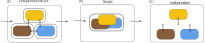
\includegraphics[width=\textwidth]{img/EDLA/community_strategies.pdf}
    \caption{Différents types de stratégies pour construire un modèle de communauté. (a) Dans le modèle compartimentalisé, chaque bactérie possède son propre compartiment cytosolique et extracellulaire. Un compartiment extracellulaire commun à l'ensemble des bactéries est également disponible. (b) Dans le modèle soupe, les bactéries sont assemblées en une seul pour former un supra-organisme. (c) Les bactéries ont chacun leur propre compartiment cytosolique mais partagent un milieu extracellulaire commun.}
    \label{fig:community-type}
\end{figure}


En fonction du type de représentation du modèle de communauté il existe plusieurs outils de modélisation de communautés microbiennes \citep{Colarusso2021}. Dans Henry et al \citep{Henry2016}, les auteurs ont choisi de maximiser une fonction de biomasse communautaire se basant sur la composition des réactions de biomasse de chaque taxon présent dans la communauté. Microbiome modeling toolbox \citep{Baldini2019}, MiCOM \citep{diener2020} et SteadyCom \citep{Chan2017} maximisent tous la somme des flux de la fonction de biomasse de chaque organisme et permettent l'étude de plus grandes communautés.  cFBA \citep{Khandelwal2013} ou encore Koch et al, \citep{Koch2016} permettent une analyse sur de petites communautés. Enfin, dans la catégorie d'une optimisation à plusieurs niveaux, on peut retrouver les outils suivants : OptCom \citep{Zomorrodi2012}, NECom \citep{Cai2020}, maximisant les fonctions de biomasse de chaque modèle individuel puis les flux de production de biomasse à l'échelle de la communauté. Pour des raisons de coût calculatoire, appliquer ces outils sur des grandes communautés microbiennes est non réalisable. \\

Toutes ces méthodes basées sur des contraintes permettent d'étudier le métabolisme et par conséquent peuvent être utilisées pour mettre en évidence l'impact positif (coopération) ou négatif (compétition) d'une interaction bactérienne. En effet, dans \citep{Freilich2011} les scores de potentiels de coopération et de compétition sont inférés en caractérisant les relations de donneurs-receveurs et de gagnants-perdants au sein de l'écosystème. Plus récemment, MMinte \citep{Mendes-Soares2016} prédit l'impact positif ou négatif d'une espèce sur une autre en comparant les croissances des espèces seules et lorsqu'elles sont en interactions deux à deux. L'analyse des interactions deux à deux ne permet pas de déduire l'ensemble des comportements de la communauté bactérienne puisque de nouvelles interactions se produisent, disparaissent ou encore se conservent \citep{Morin2022}. SMETANA \citep{Zelezniak2015} et MiCOM \citep{diener2020} contournent cette limite et proposent d'étudier les interactions bactériennes de l'ensemble des espèces de la communauté.  SMETANA définit la coopération via le potentiel d'interaction métabolique (MIP) représentant le nombre de maximal de composés nutritifs essentiels que la communauté peut produire au moyen des interactions bactériennes. La compétition est  estimée par le maximum de chevauchement de métabolites (MRO) au sein du milieu minimum pour la croissance de toutes les espèces. MiCOM ne permet pas d'obtenir directement une mesure de la coopération et de la compétition mais, tout comme SMETANA, donne une liste de métabolites potentiellement échangés avec pour chaque, le flux d'export et d'import.\\

\subsubsection{Analyse dynamique sous contraintes}
Les méthodes précédentes permettent d'analyser des communautés microbiennes de taille variable de manière statique. Or,  un écosystème est un environnement dynamique dans lequel la composition taxonomique et la quantité de ressources disponibles fluctuent au cours du temps. Une liste de méthodes, prenant en compte la temporalité dans un écosystème, ainsi que leurs limites est proposée dans les paragraphes suivants. \\

La méthode DMMM \citep{Zhuang2011} utilise des équations différentielles ordinaires pour décrire la loi de conservation de la masse pour tous les métabolites échangés et la production de biomasse de chaque espèce au sein de la communauté. Le temps est alors discrétisé, et à chaque pas de temps, une optimisation est faite. La concentration des métabolites disponibles dans le milieu extra-cellulaire est ajustée après la consommation et la production des différents métabolites échangés ainsi que la densité cellulaire (méthode explicite d'Euler). Avec ce choix temporel d'ajuster la concentration des métabolites extra-cellulaires après l'importation des nutriments, le modèle peut prédire que les espèces consomment un nutriment dont sa concentration n'est pas suffisante par rapport la densité cellulaire prédite par le modèle. Une première possibilité consiste à rendre indisponible tous les métabolites dont la concentration est négative. Une seconde possibilité revient à diminuer l'intervalle de temps entre deux calcul. En revanche, cela augmenterait le temps calculatoire.  Par exemple, $\mu$bialSim \citep{Popp2020} solutionne ce problème en réduisant le pas de temps seulement lorsque la concentration d'un métabolite échangé est négative.  \\

Les modèles dynamiques de communautés doivent prendre en compte le cas où il n'y a pas de solutions possibles pour le système dynamique étudié; on parle de résolution non faisable, ou bien, lorsqu'il y a pas un flux unique de production ou de consommation pour un métabolite. La faisabilité d'un modèle est liée à la quantité de nutriments limitants disponibles pour le système. DFBALab \citep{Gomez2018} tente de résoudre ces deux problèmes en priorisant le choix des métabolites d'intérêts à maximiser. Ainsi, une unique solution est trouvée par le solveur linéaire permettant d'outrepasser la seconde contrainte. En revanche, l'utilisateur ou l'utilisatrice doit donner une liste de métabolites échangés en amont pour que le résultat de la simulation reste cohérent. En plus, cela suppose une bonne connaissance du système biologique d'étude pour effectuer ce choix et est donc peu recommandé pour l'étude de communauté à grande échelle. D'autres méthodes existent utilisant une approche de résolution plus précise (Runge-Kutta explicite), mais plus coûteuse en temps de calcul que celle d'Euler explicite. \citep{Schroeder2020}. ou encore, un optimisation à deux niveaux \citep{Zomorrodi}, ne nécessitant pas l'intervention d'une connaissance \textit{a priori} du système d'étude. \\

%% Note à moi meme, plus précise car pour un rungekunta d'ordre 4, si on divise le pas de temps par 2, l'erreur à la fin est divisé par 16 (2^4)


Une des limites fondamentales de ces utilisations est que tous les échanges métaboliques sont conditionnés par l'optimisation de la fonction de biomasse. Ainsi, un ensemble de métabolites pouvant être échangés au sein d'une communauté mais n'étant pas essentiel pour la biomasse d'un individu ne sera donc pas identifié. Dans les travaux de Zomorrodi et al \citep{Zomorrodi2017}, ce problème est abordé en ajoutant des contraintes supplémentaires qui pré-traitent différentes stratégies comme la prise en compte de métabolites échangés coûteux. En revanche, identifier l'ensemble des stratégies à l'échelle d'une communauté ne semble pas être réalisable. Au sein de l'outil NECom \citep{Cai2020}, se basant sur une optimisation à deux niveaux, les auteurs relâchent les contraintes de flux acceptant plus de métabolites potentiellement échangés. \\

\subsection{Applications}
En plus de l'étude des interactions au sein de communautés bactériennes, la création de communautés synthétiques semble être un secteur prometteur. En effet, elle permet (1) d'identifier des communautés microbiennes d'intérêt à partir d'une liste de bactéries candidates, (2) d'évaluer l'impact d'une modification génétique sur la synergie de la communauté, et enfin (3), d'évaluer les perturbations dans le milieu de culture ou dans la composition de la biomasse sur la communauté. Dans \citep{Chiu2014}, l'utilisation d'un modèle dynamique a permis de mettre en avant une communauté composée de deux espèces qui produisent et échangent des composés uniquement lorsqu'elles sont en co-culture. Ou encore, dans \citep{Zuniga2020}, le modèle dynamique sélectionne des souches phototrophes partenaires prometteuse pour la biotechnologie durable. D'autres méthodes, comme par exemple OptAux, s'intéressent à la création de souches auxotrophes, c'est à dire ne pouvant synthétiser un composé par elles mêmes, qui sont vérifiables expérimentalement \citep{Lloyd2019}. Un autre point de vue d'analyse est celui du milieu de culture, comme par exemple dans \citep{Klitgord2010}, où l'objectif est de sélectionner un milieu de culture permettant d'observer soit des interactions du type mutualisme ou du commensalisme entre des paires d'organismes, soit une production de métabolites cibles \citep{Pacheco2021}. Dans le même esprit, FLYCOP \citep{Garcia-Jimenez2018} créé un consortium à partir d'un milieu de culture dans le but de trouver tous les échanges métaboliques permettant la production de bio-plastique. Dans \citep{Machado2021},  l'impact  \textit{in silico} de facteurs abiotiques (introduction d'une nouvelle espèce) et biotiques (disponibilité des nutriments) sur la communauté a été analysée. Ils ont montré que les communautés compétitives étaient plus sensibles aux perturbations abiotiques, et qu'en revanche, les communautés coopératives se sont révélées être sensible à l'introduction d'une nouvelle espèce. \\

Toutes ces méthodes permettent d'analyser des communautés microbiennes sous différents point de vue : identification statique ou dynamique des interactions métaboliques au sein d'une communauté donnée, recherche d'un milieu de culture pour la création d'une communauté avec le comportement souhaité, compréhension détaillée de mécanismes métaboliques intra-cellulaires ou encore, impact d'une perturbation sur le potentiel métabolique de la communauté. Malgré la précision numérique que l'on obtient, l'utilisation de ces modèles ne permet pas une analyse sur des communautés naturelles notamment en raison de la combinatoire exponentielle des échanges métaboliques. Il existe des méthodes qualitatives, s'appliquant à l'échelle d'une communauté, sacrifiant la précision numérique pour permettre résolution de ce problème combinatoire sur des communautés naturelles. 

\begin{figure}
    \centering
    \includegraphics{example-image-a}
    \caption{Review des methodes numériques pour une bactéries/communauté avec avantages et inconvéniants. Mettre si cela peut répondre à notre défis : utiliser à grande echelle, mettre en avant les interactions etc}
    \label{fig:my_label}
\end{figure}

\subsection{Méthodes et modèles qualitatifs de l'étude d'une communauté bactérienne}
Comme pour les méthodes quantitatives, les approches qualitatives en communauté se sont focalisées sur l'étude des interactions bactériennes. Nous allons voir les stratégies des approches par l'étude de graphe et par le raisonnement permettant l'identification des potentiels de coopération et de compétition au sein de communautés microbiennes de tailles variables. Pour rappel, un échange métabolique se traduit par la production d'un composé par un microorganisme dans l'environnement nutritionnel qui est lui-même consommé par un autre impactant ou non sa croissance \citep{Faust2012}. La compétition se traduit par une co-consommation d'un nutriment limitant ayant des effets néfastes sur la croissance ou sur le potentiel métabolique. La coopération et la compétition sont des mécanismes biologiques centraux pour mieux comprendre comment une communauté bactérienne fonctionne. \\


\subsubsection{Approches basées sur les graphes}
Certaines approches étudient la structure de réseaux métaboliques, sous forme d'un graphe, en déterminant la relation de dépendance des éléments du graphe au milieu nutritif. Les éléments identifiés sont donc utilisés comme une approximation des métabolites échangés \citep{Levy}. Ainsi, en se basant sur le principe d'écologie inversée consistant à déduire des processus écologiques en utilisant les données génomiques massive, la détection de potentiels de coopération et de compétition est possible. Un moyen de calculer ces potentiels  au sein d'une communauté bactérienne est de déterminer la composition nutritionnelle (graines) requise pour la communauté \citep{Carr2012}. Dans le but de quantifier la complémentarité entre toutes les paires d'espèces possibles, NetCooperate \citep{Levy2015} mesure à la fois la capacité d'un organisme hôte à répondre aux besoins nutritionnels d'un parasite endosymbiothique (BSS score) et quantifie l'aide mutuelle de deux organismes en fournissant un indice de potentiel syntrophique (MCI score). En se basant sur une analyse du milieu nutritionnel théorique, on peut également déterminer un indice de compétition métabolique en analysant les composés connectés à plusieurs organismes \citep{Levy2013}. Ainsi, NetCompt estime le potentiel de compétition en se basant sur le chevauchement métabolique \citep{Kreimer2012}. Toutes ces méthodes sont limitées à une analyse par paire d'organismes ne reflétant pas le réel potentiel coopératif ou compétitif d'une communauté microbienne complexe mais informant l'impact d'un individu sur un autre. 


\subsubsection{Modèle basés sur le raisonnement}
On a vu dans une sous section précédente que la méthode par raisonnement pouvait identifier des composés potentiellement productibles et consommables. Les travaux de \citep{Frioux2018} ont décrit un modèle de communauté basé sur la raisonnement en incorporant la notion de réversibilité des réactions, une première définition de la coopération. Grâce à leur outil développé, MISCOTO, ils peuvent également sélectionner des communautés sous la contrainte de taille minimale de la communauté finale. MISCOTO a été élargis dans \citep{Belcour.2020} identifient des interactions positives au moyen d'un raisonnement logique en développant l'outil Metage2Metabo. Il permet d'identifier la valeur ajoutée de la coopération métabolique au sein d'une communauté au moyen du métabolisme de chaque individu, et identifier et cribler des espèces d'intérêts parmi tous les membres de la communauté.

\begin{figure}[h!]
    \centering
    \includegraphics[width=\textwidth]{img/EDLA/review-methode.pdf}
    \caption{Liste non exhaustives des methodes qualitatives pour analyser une bactérie et des communautés avec leurs avantages et inconvéniants. Extrait de Cerk et al. \textit{Community-scale models of microbiomes: articulating metabolic modelling and metagenome sequencing}, 2023,Environmental Microbiology.[en révision]}
    \label{fig:my_label}
\end{figure}

\subsection{Défis rencontrés lors de l'analyse de la modélisation qualitative et quantitative du métabolisme des communautés}
Des questions similaires à celles déjà rencontrées (voir la sous section \ref{defi}) se posent également au niveau de la communauté. Les ensembles de métabolites produits en intracellulaire peuvent être disponibles pour l'ensemble des membres de la communauté. En effet, nous savons que les cellules sont capables de lyse cellulaire, libérant ainsi tous les produits métaboliques dans le milieu extra-cellulaire \citep{Fazzino2020}. De plus, les fuites métaboliques passives, c'est à dire sans coût énergétique pour la cellule, ont été montrées comme étant dominantes dans les interactions microbiennes  \citep{Pacheco.2019m3q}. Une seconde notion à prendre en compte est celle de la frontière des compartiments métaboliques propre à chaque espèce de la communauté. 


\section*{Conclusion}
Dans ce chapitre, nous avons proposé une revue de la littérature sur la thématique de la modélisation du métabolisme, en présentant dans un premier temps une définition et différentes représentations d'un réseau métabolique. Et dans un second temps, une collection de méthodes quantitatives et qualitatives d'analyse du métabolisme à l'échelle d'une cellule et d'un écosystème bactérien a été détaillé.\\
Parmi les approches de modélisation du métabolisme, nous avons vu que les modèles numériques sont pertinents d'une part, pour leurs capacités à intégrer des types de données omiques au moyen de contraintes linéaires ou d'optimisation, et d'autre part, pour la précision numérique qu'ils offrent. Cependant, cette aptitude rend délicate leur utilisation à des communautés plus complexes pour des raisons de coûts, calculatoire et du temps passé par le modélisateur ou de la modélisatrice, et de disponibilités de données. \\
De façon alternative, l'approche par raisonnement de l'étude du métabolisme dépasse ces limites en faisant une abstraction booléenne du métabolisme. De plus, nous avons vu que cette approche par raisonnement fournit une explicabilité aux modèles. En revanche, la précision apportée par ces modèles reste néanmoins qualitative. \textit{In fine}, il existe pas de méthode universelle permettant de répondre à notre objectif, et un compromis doit être fait. Dans le reste de ce manuscrit, nous essayerons de mieux comprendre les apports et les enjeux de chaque type de modélisation dans le but de créer une approche hybride répondant à notre problématique.\\
Nous verrons ainsi, dans le chapitre \ref{ccmc}, une application de cette approche de raisonnement sur un ensemble d'écosystèmes et comment l'explicabilité d'un modèle permet de définir un score de coopération et de compétition pour une communauté donnée. \\
L'intérêt d'obtenir des modèles explicables sera particulièrement exploité au cours du chapitre \ref{enrichissement} consistant à (i) sélectionner un ensemble de communauté potentiellement d'intérêt à partir d'une ensemble de contraintes, (ii) intégrer une temporalité. \\
Enfin, les données nécessaire pour réaliser ces travaux se sont uniquement basés sur des données génomiques. Dans le cas idéal, plusieurs types de données omiques permettent d'apporter des informations à différents échelles du métabolisme. Ainsi, nous verrons au cours du chapitre \ref{tango}, la plus value des données multi-omiques sur l'analyse du métabolisme d'une communauté contrôlé composée de trois bactéries et le degré de précision que l'on peut obtenir concernant les mécanismes intercellulaires.

\end{document} %